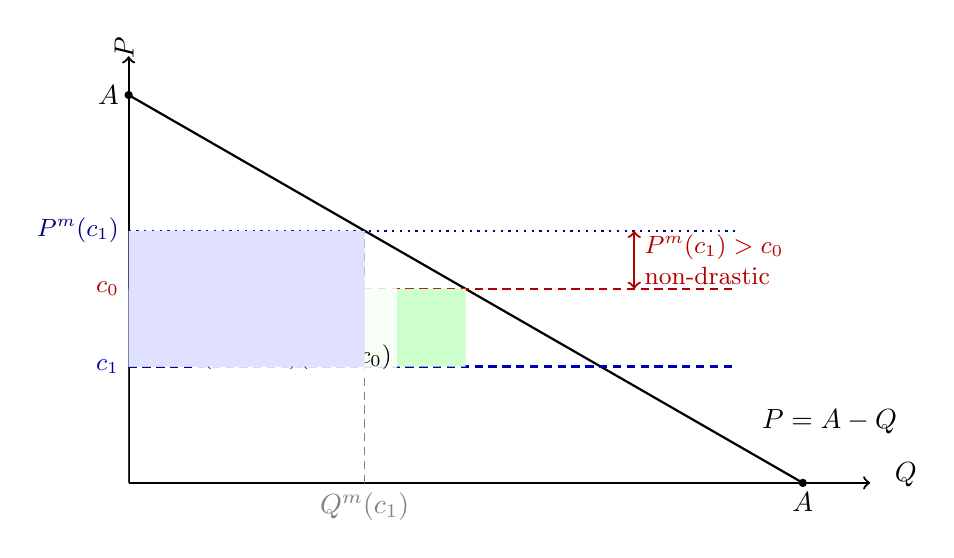
\begin{tikzpicture}
\begin{axis}[
  width=11cm, height=7cm,
  xmin=0, xmax=22,
  ymin=0, ymax=22,
  axis lines=left,
  axis line style={thick, ->},
  ticks=none,
  clip=false,
  xlabel={$Q$},
  ylabel={$P$},
  xlabel style={at={(axis description cs:1.02,0.02)}, anchor=west},
  ylabel style={at={(axis description cs:0.02,1.02)}, anchor=south},
]

% Parameters: A=20, c0=10, c1=6
\pgfmathsetmacro{\A}{20}
\pgfmathsetmacro{\cO}{10}
\pgfmathsetmacro{\cI}{6}
% Monopoly with c1: Q^m = (A-c1)/2 = 7, P^m = (A+c1)/2 = 13
\pgfmathsetmacro{\Qm}{(\A-\cI)/2}
\pgfmathsetmacro{\Pm}{(\A+\cI)/2}

% Demand curve: P = A - Q
\addplot[thick, domain=0:\A, samples=2, color=black] {\A - x};
\node[anchor=south west] at (axis cs:18.5,2) {$P = A - Q$};

% Cost lines
\addplot[thick, densely dashed, domain=0:18, samples=2, color=red!70!black] {\cO};
\node[anchor=east, color=red!70!black, font=\small] at (axis cs:0,\cO) {$c_0$};

\addplot[thick, densely dashed, domain=0:18, samples=2, color=blue!70!black] {\cI};
\node[anchor=east, color=blue!70!black, font=\small] at (axis cs:0,\cI) {$c_1$};

% Monopoly price with c1
\addplot[thick, dotted, domain=0:18, samples=2, color=blue!50!black] {\Pm};
\node[anchor=east, color=blue!50!black, font=\small] at (axis cs:0,\Pm) {$P^m(c_1)$};

% Vertical dashed at Q^m(c1)
\addplot[densely dashed, thin, gray] coordinates {(\Qm,0) (\Qm,\Pm)};
\node[anchor=north, gray] at (axis cs:\Qm,0) {$Q^m(c_1)$};

% Shade non-drastic profit: rectangle from c1 to c0, width A-c0
% Innovator limit-prices at c0, sells Q = A - c0 = 10
\pgfmathsetmacro{\Qpc}{\A - \cO}
\addplot[fill=green!20, draw=none, forget plot]
  coordinates {(0,\cI) (\Qpc,\cI) (\Qpc,\cO) (0,\cO)} \closedcycle;

% Label the non-drastic profit rectangle
\node[align=center, fill=white, fill opacity=0.85, text opacity=1, inner sep=2pt, font=\small] at (axis cs:5,8) {Non-drastic\\profit\\$(c_0 - c_1)(A-c_0)$};

% Shade monopoly profit area (triangle-like) with c1
% Rectangle from c1 to P^m(c1), width Q^m(c1)
\addplot[fill=blue!12, draw=none, forget plot]
  coordinates {(0,\cI) (\Qm,\cI) (\Qm,\Pm) (0,\Pm)} \closedcycle;

% Annotation: P^m(c1) > c0 means non-drastic
\draw[thick, <->, color=red!70!black]
  (axis cs:15,\cO) -- (axis cs:15,\Pm)
  node[midway, right, align=left, font=\small] {$P^m(c_1) > c_0$\\non-drastic};

% Mark key points
\fill (axis cs:0,\A) circle (1.5pt);
\node[anchor=east] at (axis cs:0,\A) {$A$};

\fill (axis cs:\A,0) circle (1.5pt);
\node[anchor=north] at (axis cs:\A,0) {$A$};

\end{axis}
\end{tikzpicture}
